% Onco-TTT: AI-Powered Cancer Hypothesis Generation
% Scientific Preprint — February 2026
% Compiled with tectonic (XeLaTeX-based)
\documentclass[11pt,a4paper]{article}

% ── Packages ──────────────────────────────────────────────────────
\usepackage[margin=2.5cm]{geometry}
\usepackage[utf8]{inputenc}
\usepackage[T1]{fontenc}
\usepackage{lmodern}
\usepackage{microtype}
\usepackage{amsmath,amssymb}
\usepackage{graphicx}
\usepackage{xcolor}
\usepackage{booktabs}
\usepackage{tabularx}
\usepackage{multirow}
\usepackage{enumitem}
\usepackage{float}
\usepackage{caption}
\usepackage{subcaption}
\usepackage[colorlinks=true,linkcolor=blue!60!black,citecolor=blue!60!black,urlcolor=blue!60!black]{hyperref}
\usepackage{tikz}
\usepackage{pgfplots}
\pgfplotsset{compat=1.18}
\usetikzlibrary{arrows.meta,positioning,shapes.geometric,fit,backgrounds,calc,decorations.pathreplacing,shadows}

% ── Colors (matched to concepts per Saloni's guidelines) ─────────
\definecolor{compute}{HTML}{3b82f6}    % blue: internal compute steps
\definecolor{externalapi}{HTML}{10b981} % green: external APIs/data
\definecolor{outputpurple}{HTML}{7c3aed}% purple: outputs/results
\definecolor{userinput}{HTML}{1e293b}   % dark: user-facing elements
\definecolor{genecol}{HTML}{3b82f6}     % gene entities
\definecolor{diseasecol}{HTML}{ef4444}  % disease entities
\definecolor{drugcol}{HTML}{10b981}     % drug entities
\definecolor{pathwaycol}{HTML}{8b5cf6}  % pathway entities
\definecolor{mutationcol}{HTML}{f59e0b} % mutation entities
\definecolor{cautionamber}{HTML}{f59e0b}
\definecolor{failred}{HTML}{ef4444}
\definecolor{passgreen}{HTML}{10b981}
\definecolor{unknowngray}{HTML}{9ca3af}

% ── Metadata ──────────────────────────────────────────────────────
\title{\textbf{Onco-TTT: An Open-Source Platform for Automated\\Cancer Hypothesis Generation via Entity Extraction,\\Knowledge Graphs, and Multi-Source Validation}}
\author{Ashish Makani\\
\small Ashoka University, Sonipat, India\\
\small \texttt{ashish.makani@ashoka.edu.in}}
\date{February 2026 \quad $\cdot$ \quad Preprint (not peer-reviewed)}

% ══════════════════════════════════════════════════════════════════
\begin{document}
\maketitle

% ── Abstract ──────────────────────────────────────────────────────
\begin{abstract}
We present \textbf{Onco-TTT}, an open-source web platform that generates testable cancer research hypotheses from free-text queries.
The system chains four stages:
(1)~zero-shot biomedical named entity recognition using GLiNER2 to extract genes, diseases, drugs, pathways, and six additional entity types;
(2)~knowledge graph construction enriched by the OpenTargets GraphQL~API;
(3)~graph-based activation propagation to rank query-relevant nodes; and
(4)~structured hypothesis assembly from graph topology.
In parallel, the platform retrieves supporting literature from Semantic Scholar, single-cell metadata from the CZI CELLxGENE Census, and runs a six-dimensional validation dashboard that cross-references DepMap gene essentiality, cBioPortal survival data, GTEx tissue expression, ClinicalTrials.gov trial counts, and OpenTargets tractability.
Additional modules provide AlphaFold structure analysis with geometric pocket detection, USPTO patent landscape scoring, cell line recommendations, and CRISPR guide RNA design.
Onco-TTT is deployed at \url{https://onco-hypothesis.up.railway.app} with source code at \url{https://github.com/inventcures/oncology_hypothesis_generation}.

\medskip
\noindent\textbf{Transparency statement.}
Internal module names in this paper (``ARK'' for the KG pipeline, ``TTT'' for activation propagation) are project codenames, not references to published methods.
The activation propagation step is a simplified graph diffusion heuristic, not neural test-time training.
Single-cell atlas coordinates are synthetically generated.
Validation modules use curated fallback data when live APIs are unavailable.
\end{abstract}

% ── 1. Introduction ───────────────────────────────────────────────
\section{Introduction}

Cancer research generates vast quantities of genomic, transcriptomic, and clinical data across fragmented databases.
A researcher investigating, for example, \textit{``KRAS G12C resistance mechanisms in NSCLC,''} must manually query OpenTargets for gene-disease associations, search Semantic Scholar for relevant literature, check DepMap for gene essentiality, assess clinical trial competition on ClinicalTrials.gov, and evaluate druggability---each through a separate interface with its own query syntax.

Onco-TTT automates this workflow.
Given a free-text oncology query, the platform extracts biological entities, constructs an enriched knowledge graph, generates ranked hypotheses, retrieves supporting evidence from multiple public databases, and presents all results in a unified interactive interface.

The system makes three practical contributions:
\begin{enumerate}[nosep]
    \item A modular, open-source pipeline that chains zero-shot NER, knowledge graph enrichment, literature search, and multi-source validation into a single query-to-hypothesis workflow.
    \item A six-dimensional validation dashboard that provides immediate evidence grounding for generated hypotheses.
    \item An interactive web interface with knowledge graph visualization, entity tables, paper retrieval, and feasibility assessment tools including structural analysis and CRISPR protocol generation.
\end{enumerate}

\noindent
We are transparent about what Onco-TTT is and is not.
It is an \emph{integration platform} that combines established methods and public data sources.
It does not introduce novel machine learning architectures.
Its hypotheses are heuristic, assembled from graph topology rather than from a fine-tuned language model, and have not been systematically benchmarked against ground truth.
We describe the system accurately so that researchers can evaluate its utility for their own work.

% ── 2. System Architecture ────────────────────────────────────────
\section{System Architecture}

Onco-TTT is a two-service web application: a Python/FastAPI backend and a TypeScript/Next.js~14 frontend, deployed on Railway.
The backend exposes 12 REST endpoints.
The main \texttt{/generate} endpoint runs three tasks concurrently via \texttt{asyncio.gather}: knowledge graph construction, literature search, and single-cell atlas retrieval.
Individual task failures are isolated (\texttt{return\_exceptions=True}), ensuring partial results are always returned.

Figure~\ref{fig:pipeline} shows the end-to-end pipeline architecture.

% ── Figure 1: Pipeline Architecture (TikZ) ───────────────────────
% Following Saloni: horizontal text, direct labels, color matched to
% concept (blue=compute, green=external, purple=output, dark=input),
% standalone with legend.
\begin{figure}[htbp]
\centering
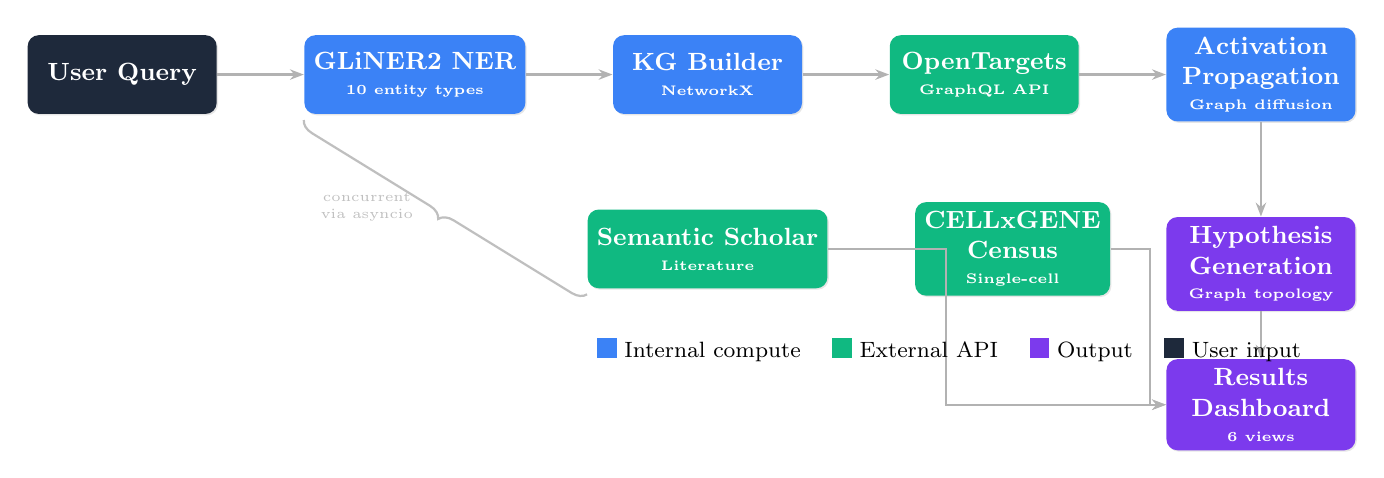
\begin{tikzpicture}[
    node distance=0.6cm and 1.1cm,
    block/.style={rectangle, rounded corners=4pt, minimum height=1.0cm, minimum width=2.4cm, font=\small\bfseries, text=white, align=center, drop shadow={shadow xshift=0.5pt, shadow yshift=-0.5pt, opacity=0.2}},
    inputblock/.style={block, fill=userinput},
    compblock/.style={block, fill=compute},
    apiblock/.style={block, fill=externalapi},
    outblock/.style={block, fill=outputpurple},
    arr/.style={-{Stealth[length=5pt]}, thick, color=gray!60},
    ann/.style={font=\tiny\color{gray!70}, align=center},
]

% Row 1: Main pipeline
\node[inputblock] (query) {User Query};
\node[compblock, right=of query] (gliner) {GLiNER2 NER\\[-2pt]{\tiny 10 entity types}};
\node[compblock, right=of gliner] (kg) {KG Builder\\[-2pt]{\tiny NetworkX}};
\node[apiblock, right=of kg] (ot) {OpenTargets\\[-2pt]{\tiny GraphQL API}};
\node[compblock, right=of ot] (prop) {Activation\\Propagation\\[-2pt]{\tiny Graph diffusion}};

\draw[arr] (query) -- (gliner);
\draw[arr] (gliner) -- (kg);
\draw[arr] (kg) -- (ot);
\draw[arr] (ot) -- (prop);

% Row 2: Parallel tasks
\node[apiblock, below=1.2cm of kg] (s2) {Semantic Scholar\\[-2pt]{\tiny Literature}};
\node[apiblock, right=of s2] (census) {CELLxGENE\\Census\\[-2pt]{\tiny Single-cell}};

% Row 3: Outputs
\node[outblock, below=1.2cm of prop] (hyp) {Hypothesis\\Generation\\[-2pt]{\tiny Graph topology}};
\node[outblock, below=of hyp] (dash) {Results\\Dashboard\\[-2pt]{\tiny 6 views}};

% Arrows
\draw[arr] (prop) -- (hyp);
\draw[arr] (hyp) -- (dash);
\draw[arr] (s2.east) -- ++(1.5,0) |- (dash.west);
\draw[arr] (census.east) -- ++(0.5,0) |- (dash.west);

% Concurrent bracket
\draw[decorate, decoration={brace, amplitude=5pt, mirror}, thick, gray!50]
    ([yshift=-2pt]gliner.south west) -- ([yshift=-2pt]s2.south west)
    node[midway, left=8pt, ann] {concurrent\\via asyncio};

% Legend — horizontal, at bottom
\node[anchor=north west, font=\footnotesize] at ([yshift=-0.5cm]s2.south west) {
    \tikz{\fill[compute] (0,0) rectangle (0.25,0.25);} Internal compute \quad
    \tikz{\fill[externalapi] (0,0) rectangle (0.25,0.25);} External API \quad
    \tikz{\fill[outputpurple] (0,0) rectangle (0.25,0.25);} Output \quad
    \tikz{\fill[userinput] (0,0) rectangle (0.25,0.25);} User input
};

\end{tikzpicture}
\caption{\textbf{Onco-TTT pipeline architecture.} A free-text oncology query flows through entity extraction, knowledge graph construction with OpenTargets enrichment, and graph-based activation propagation to produce ranked hypotheses. Literature search and atlas retrieval run concurrently. All results are merged into a six-view interactive dashboard.}
\label{fig:pipeline}
\end{figure}


% ── 3. Methods ────────────────────────────────────────────────────
\section{Methods}

\subsection{Entity Extraction}
\label{sec:ner}

Onco-TTT uses GLiNER2~\cite{zaratiana2023gliner}, a generalist NER model based on a bidirectional transformer encoder, to extract biological entities from free-text queries in a zero-shot setting.
We define a 10-type oncology entity schema (Table~\ref{tab:entities}) and a 10-type relation schema covering interactions such as \textit{targets}, \textit{drives}, \textit{mutated\_in}, and \textit{synergizes\_with}.

The model (\texttt{fastino/gliner2-base-v1}) is loaded once as a thread-safe singleton.
Extraction results are cached in an LRU cache (500~entries, 30-minute TTL) keyed by SHA-256 hash of normalized input text.
The confidence threshold is 0.4 for entities and 0.3 for research focus classification.

% ── Table 1: Entity Types ─────────────────────────────────────────
% Following Saloni: ordered logically, horizontal text, clear headers.
\begin{table}[htbp]
\centering
\caption{\textbf{Oncology entity types} extracted by GLiNER2 in zero-shot mode. Types are grouped by biological category.}
\label{tab:entities}
\small
\begin{tabularx}{\linewidth}{@{}l l X@{}}
\toprule
\textbf{Category} & \textbf{Entity type} & \textbf{Description} \\
\midrule
\multirow{2}{*}{Molecular} & Gene & Gene symbols (e.g., KRAS, TP53, EGFR) \\
 & Mutation & Specific variants (e.g., G12C, T790M, V600E) \\
\midrule
\multirow{2}{*}{Clinical} & Disease & Cancer types and subtypes \\
 & Drug & Therapeutic agents (e.g., osimertinib, sotorasib) \\
\midrule
\multirow{2}{*}{Biological} & Pathway & Signaling pathways (e.g., MAPK, PI3K/AKT) \\
 & Mechanism & Biological processes (e.g., apoptosis, EMT) \\
\midrule
\multirow{2}{*}{Cellular} & Cell type & Cell populations (e.g., T~cells, macrophages) \\
 & Biomarker & Predictive or prognostic markers \\
\midrule
\multirow{2}{*}{Anatomical} & Anatomical site & Tissue/organ locations \\
 & Clinical outcome & Endpoints (e.g., overall survival, response) \\
\bottomrule
\end{tabularx}
\end{table}

\subsection{Knowledge Graph Construction}
\label{sec:kg}

Extracted entities and relations are assembled into a directed graph (\texttt{networkx.DiGraph}).
Each node stores its entity type, extraction confidence, and a deterministic color assignment (Table~\ref{tab:entities}).
Each edge stores its relation type, label, weight (from extraction confidence), and a corresponding color.

The graph is then enriched via the OpenTargets Platform GraphQL API~\cite{ochoa2023opentargets}.
Starting from the highest-confidence gene entity (or a regex fallback \texttt{[A-Z][A-Z0-9]\{2,7\}}), the system:
\begin{enumerate}[nosep]
    \item Queries \texttt{search(queryString, entityNames: ["target","disease"])} to resolve the entity to an Ensembl or EFO identifier.
    \item Fetches the top-10 associated diseases (for gene seeds) or targets (for disease seeds) via \texttt{associatedDiseases} or \texttt{associatedTargets}.
    \item Adds curated pathway edges for 15 common oncogenes (e.g., KRAS$\rightarrow$RAS/MAPK, BRCA1$\rightarrow$Homologous Recombination) and cell-type context for 7 genes.
\end{enumerate}

Node visual importance is computed as $0.4 \times \text{degree\_centrality} + 0.6 \times \text{confidence}$, mapped to a radius between 22 and 38~pixels.
Layout is computed via the Fruchterman--Reingold spring algorithm (80~iterations, seed~42 for reproducibility).

\subsection{Activation Propagation}
\label{sec:ttt}

After graph construction, a graph diffusion step ranks nodes by query relevance.
Nodes whose labels contain query terms receive an initial activation of~1.0.
For $k=5$ iterations, activation propagates to neighbors weighted by edge weight and a learning rate $\eta=0.1$:
\[
a_v^{(t+1)} = a_v^{(t)} + \eta \sum_{u \in \mathcal{N}^{-}(v)} a_u^{(t)} \cdot w_{uv}
\]
where $\mathcal{N}^{-}(v)$ denotes in-neighbors of node $v$ and $w_{uv}$ is the edge weight.
The top-10 nodes by final activation score are returned.

\textbf{Transparency note.}
This module is internally named ``TTT'' after the Test-Time Training concept~\cite{sun2024ttt}, which adapts neural network parameters at inference time.
Our implementation is a simplified graph diffusion heuristic---it performs label propagation on a static graph, not gradient-based parameter adaptation.
The name reflects an aspirational design direction.

\subsection{Hypothesis Generation}
\label{sec:hypotheses}

Hypotheses are assembled deterministically from the knowledge graph topology using four strategies:
\begin{enumerate}[nosep]
    \item \textbf{Gene--disease driver:} For each gene node, find linked disease nodes; the strongest association (by edge weight) becomes a ``Gene X as Driver in Disease Y'' hypothesis.
    \item \textbf{Drug--target:} For each drug node, find gene nodes connected by \textit{targets} or \textit{inhibits} relations.
    \item \textbf{Mutation--resistance:} For each mutation node, link to related mechanisms or genes to propose resistance hypotheses.
    \item \textbf{Pathway involvement:} For each pathway node, find connected genes to suggest coordinated signaling hypotheses.
\end{enumerate}
Each hypothesis receives a confidence score derived from edge weights ($\min(0.95, 0.6 + w \times 0.3)$) and a novelty score inversely related to confidence.
Results are capped at five hypotheses per query.

\subsection{Literature Search}
\label{sec:literature}

The platform queries the Semantic Scholar Academic Graph API~\cite{kinney2023s2} for papers matching the user's query.
Up to six papers are returned per request, sorted by citation count.
Retrieved fields include title, abstract (with TLDR fallback), authors (truncated to three plus ``et al.''), year, citation count, journal, DOI, PubMed ID, and open-access PDF URL.
An optional API key (\texttt{S2\_API\_KEY}) provides higher rate limits.

\subsection{Single-Cell Atlas Integration}
\label{sec:atlas}

Tissue-relevant single-cell metadata is retrieved from the CELLxGENE Census~\cite{czi2023cellxgene} via the \texttt{cellxgene\_census} Python SDK.
The system infers tissue type from the query text (9 tissue mappings, defaulting to ``lung'') and fetches up to 300 cells with metadata including cell type and disease annotation.

\textbf{Caveat.}
The UMAP coordinates displayed in the frontend are \emph{synthetically generated}---cell types receive random cluster centers with Gaussian noise---not projections from a reference atlas embedding.
Gene expression values are random placeholders.
This module provides metadata exploration, not quantitative single-cell analysis.

\subsection{Validation Dashboard}
\label{sec:validation}

The validation module runs six checks concurrently via \texttt{asyncio.gather} (Figure~\ref{fig:validation}), each scoring 0--100.
The overall score is the arithmetic mean.

% ── Figure 2: Validation Dashboard ────────────────────────────────
% Following Saloni: horizontal bars, direct labels, color matched to
% status semantics (green=pass, amber=caution, red=fail, gray=unknown),
% self-contained with title and subtitle.
\begin{figure}[htbp]
\centering
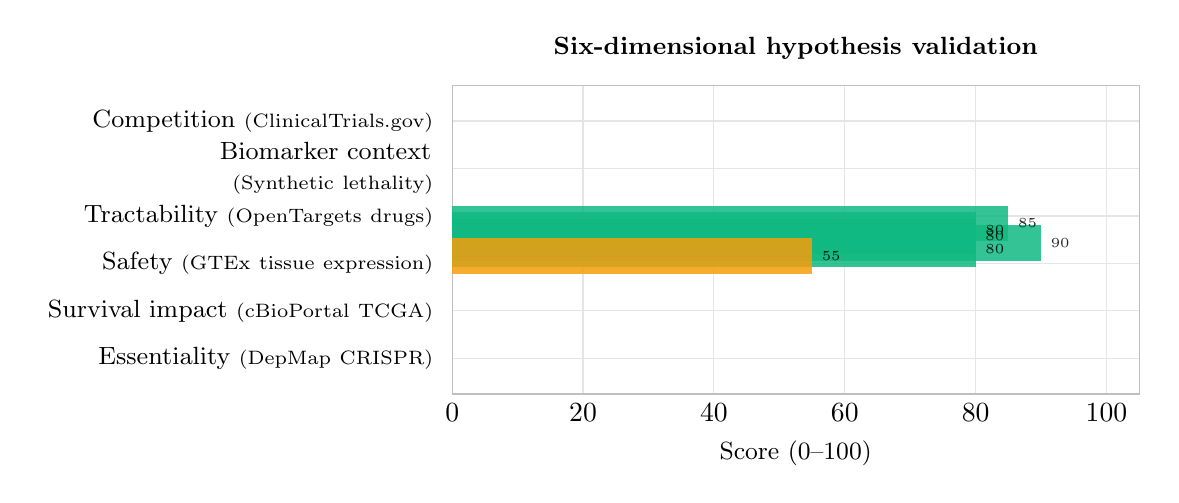
\begin{tikzpicture}
\begin{axis}[
    title={\textbf{Six-dimensional hypothesis validation}},
    title style={font=\small},
    xbar,
    width=0.85\linewidth,
    height=5.5cm,
    xlabel={Score (0--100)},
    xlabel style={font=\small},
    xmin=0, xmax=105,
    ytick={1,2,3,4,5,6},
    yticklabels={%
        {Competition \scriptsize(ClinicalTrials.gov)},%
        {Biomarker context \scriptsize(Synthetic lethality)},%
        {Tractability \scriptsize(OpenTargets drugs)},%
        {Safety \scriptsize(GTEx tissue expression)},%
        {Survival impact \scriptsize(cBioPortal TCGA)},%
        {Essentiality \scriptsize(DepMap CRISPR)}%
    },
    yticklabel style={font=\small, align=right, text width=5.0cm},
    y dir=reverse,
    bar width=0.45cm,
    nodes near coords,
    nodes near coords style={font=\tiny, anchor=west},
    every axis plot/.append style={fill opacity=0.85},
    enlarge y limits=0.15,
    grid=major,
    grid style={gray!20},
    major x tick style={draw=none},
    ytick style={draw=none},
    axis line style={gray!50},
]
% Example scores for KRAS in Lung Cancer (from curated fallback data)
\addplot[fill=passgreen, draw=none] coordinates {(85,1)};    % Essentiality
\addplot[fill=passgreen, draw=none] coordinates {(80,2)};    % Survival
\addplot[fill=passgreen, draw=none] coordinates {(80,3)};    % Safety (KRAS is tumor-selective)
\addplot[fill=passgreen, draw=none] coordinates {(90,4)};    % Tractability (sotorasib, adagrasib)
\addplot[fill=passgreen, draw=none] coordinates {(80,5)};    % Biomarker (STK11/KEAP1 co-mutations)
\addplot[fill=cautionamber, draw=none] coordinates {(55,6)};  % Competition (moderate)
\end{axis}
\end{tikzpicture}

\vspace{-0.2cm}
{\small\textit{Example: KRAS in lung adenocarcinoma. Scores use curated reference data when live APIs are unavailable. Color indicates status: {\color{passgreen}green}~=~pass, {\color{cautionamber}amber}~=~caution, {\color{failred}red}~=~fail, {\color{unknowngray}gray}~=~unknown.}}
\caption{\textbf{Validation dashboard scores.} Each bar represents one of six parallel validation checks with its data source shown in parentheses. The overall score is the arithmetic mean across all checks.}
\label{fig:validation}
\end{figure}

The six checks are:
\begin{enumerate}[nosep]
    \item \textbf{Essentiality} (DepMap): CRISPR dependency scores (Chronos). Scores below $-1.0$ indicate strong essentiality; selectivity is the difference between target and pan-cancer lineage scores.
    \item \textbf{Survival impact} (cBioPortal/TCGA): Hazard ratios from expression-survival correlation. $\text{HR} > 1.5$ with $p < 0.05$ indicates a poor-prognosis marker.
    \item \textbf{Safety} (GTEx): Normal tissue expression in 8 vital organs. Genes with TPM~$> 10$ in $\geq 3$ vital tissues receive a ``fail'' status.
    \item \textbf{Tractability} (OpenTargets): Counts of approved drugs, clinical-stage compounds, and preclinical candidates.
    \item \textbf{Biomarker context}: Curated synthetic lethality partners (e.g., PARP1$\leftrightarrow$BRCA1/2, PRMT5$\leftrightarrow$MTAP).
    \item \textbf{Competition} (ClinicalTrials.gov): Active trial counts via the v2~API. $>10$ active trials or Phase~3 entries indicate a crowded landscape.
\end{enumerate}

When live APIs are unavailable, the system falls back to curated reference data derived from published literature (10~genes with cancer-type-specific dependency scores, 8~genes with hazard ratios, 10~genes with drug data).
An LLM-powered rationale synthesis (GPT-4o-mini) integrates all six check summaries into a 2--3 sentence scientific rationale; a template-based fallback is used when no API key is configured.

\subsection{Additional Modules}
\label{sec:additional}

Four additional modules are available for hypothesis feasibility assessment:

\paragraph{Structural analysis.}
Fetches AlphaFold~\cite{jumper2021alphafold} predicted structures via UniProt ID resolution, then performs custom geometric pocket detection using neighbor density at 5/10~\AA{} cutoffs, concavity estimation, hierarchical clustering at 15~\AA{}, and convex hull volume computation.
Druggability is scored as $0.3 \times \text{size} + 0.3 \times \text{hydrophobicity} + 0.2 \times \text{confidence} + 0.2 \times \text{enclosure}$ (ideal pocket~$\approx$500~\AA$^3$).

\paragraph{Patent landscape.}
Queries the USPTO PatentsView API for patents mentioning the target gene and disease over the past 10~years.
A ``scooped score'' (0--100) combines filing volume (0--40), filing trend (0--30), and competitor count (0--30).

\paragraph{Cell line recommendations.}
Integrates Cellosaurus metadata and Cell Model Passports (Sanger/DepMap) data to recommend cell lines, with match scoring based on data richness, mutation concordance, and known problematic line flagging (e.g., HeLa cross-contamination).

\paragraph{CRISPR protocol generation.}
Retrieves coding sequences from the Ensembl REST API and designs SpCas9 guide RNAs by scanning for NGG PAM sites on both strands.
gRNA scoring incorporates GC content (40--70\% optimal), position-specific nucleotide weights (simplified Doench et~al.~2016 Rule Set~2~\cite{doench2016grna}), and penalties for poly-T termination signals and restriction enzyme sites.

% ── 4. Implementation ─────────────────────────────────────────────
\section{Implementation}

% ── Figure 3: Technology stack / data source map ──────────────────
% Following Saloni: panel layout, direct labels, color-matched to
% function category.
\begin{figure}[htbp]
\centering
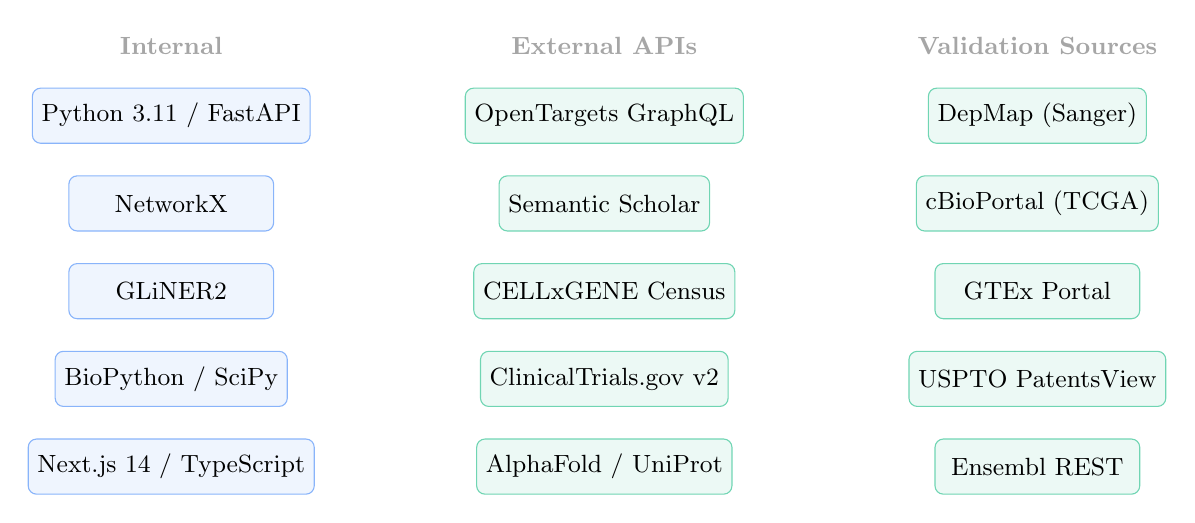
\begin{tikzpicture}[
    node distance=0.4cm,
    sbox/.style={rectangle, rounded corners=3pt, minimum height=0.7cm, minimum width=2.6cm, font=\small, align=center, draw=#1!60, fill=#1!8, text=black},
    catlab/.style={font=\small\bfseries, text=gray!70},
]

% --- Column 1: Internal ---
\node[catlab] (c1) at (0, 0) {Internal};
\node[sbox=compute, below=0.3cm of c1] (py) {Python 3.11 / FastAPI};
\node[sbox=compute, below=of py] (nx) {NetworkX};
\node[sbox=compute, below=of nx] (gl) {GLiNER2};
\node[sbox=compute, below=of gl] (bp) {BioPython / SciPy};
\node[sbox=compute, below=of bp] (ts) {Next.js 14 / TypeScript};

% --- Column 2: External APIs ---
\node[catlab] at (5.5, 0) (c2) {External APIs};
\node[sbox=externalapi, below=0.3cm of c2] (otapi) {OpenTargets GraphQL};
\node[sbox=externalapi, below=of otapi] (s2api) {Semantic Scholar};
\node[sbox=externalapi, below=of s2api] (cxg) {CELLxGENE Census};
\node[sbox=externalapi, below=of cxg] (ct) {ClinicalTrials.gov v2};
\node[sbox=externalapi, below=of ct] (af) {AlphaFold / UniProt};

% --- Column 3: Validation Sources ---
\node[catlab] at (11, 0) (c3) {Validation Sources};
\node[sbox=externalapi, below=0.3cm of c3] (dm) {DepMap (Sanger)};
\node[sbox=externalapi, below=of dm] (cbio) {cBioPortal (TCGA)};
\node[sbox=externalapi, below=of cbio] (gtex) {GTEx Portal};
\node[sbox=externalapi, below=of gtex] (pat) {USPTO PatentsView};
\node[sbox=externalapi, below=of pat] (ens) {Ensembl REST};

\end{tikzpicture}
\caption{\textbf{Technology stack and data sources.} Internal components (left) communicate with 10 external APIs (center, right) via asynchronous HTTP clients (\texttt{httpx.AsyncClient}). All external calls have curated fallback data for resilience.}
\label{fig:stack}
\end{figure}

\subsection{Backend}

The backend consists of 13~Python modules totaling approximately 6,200 lines.
Key architectural decisions include:
\begin{itemize}[nosep]
    \item \textbf{Request-scoped graph state:} Each \texttt{/generate} request creates a fresh \texttt{OncoGraph} instance to prevent concurrent state corruption, while sharing a persistent \texttt{httpx} connection pool for OpenTargets.
    \item \textbf{Concurrency:} Knowledge graph construction, literature search, and atlas retrieval run in parallel via \texttt{asyncio.gather} with \texttt{return\_exceptions=True}. Synchronous atlas operations are wrapped in \texttt{asyncio.to\_thread}.
    \item \textbf{Graceful degradation:} Every external API call has a typed exception handler and curated fallback data. A complete failure of all external APIs still produces a functional (mock-data) response.
    \item \textbf{Input validation:} All text inputs are bounded to 2,000 characters via Pydantic \texttt{Field(max\_length=2000)}.
    \item \textbf{Semantic caching:} An orchestrator module caches API results with keyword-based fuzzy matching (Jaccard similarity $> 0.8$, 1-hour TTL, 1,000 entries).
\end{itemize}

\subsection{Frontend}

The frontend is a single-page application built with Next.js~14 (App Router) and TypeScript.
The knowledge graph is rendered as pure inline SVG (no external graph library); node positions are computed server-side.
Interactive features include node/edge hover with neighbor highlighting, six switchable view modes, CSV/BibTeX export, and a Mol*-based 3D protein structure viewer.
State is managed via 21~\texttt{useState} hooks with \texttt{useCallback}/\texttt{useMemo} optimizations.

% ── 5. Example Walkthrough ────────────────────────────────────────
\section{Example Walkthrough}

We illustrate the system with the query \textit{``role of TP53 in cancer.''}

% ── Figure 4: Example KG (conceptual) ────────────────────────────
% Following Saloni: direct labels, colors matched to entity type,
% no separate legend (types labeled inline), standalone caption.
\begin{figure}[htbp]
\centering
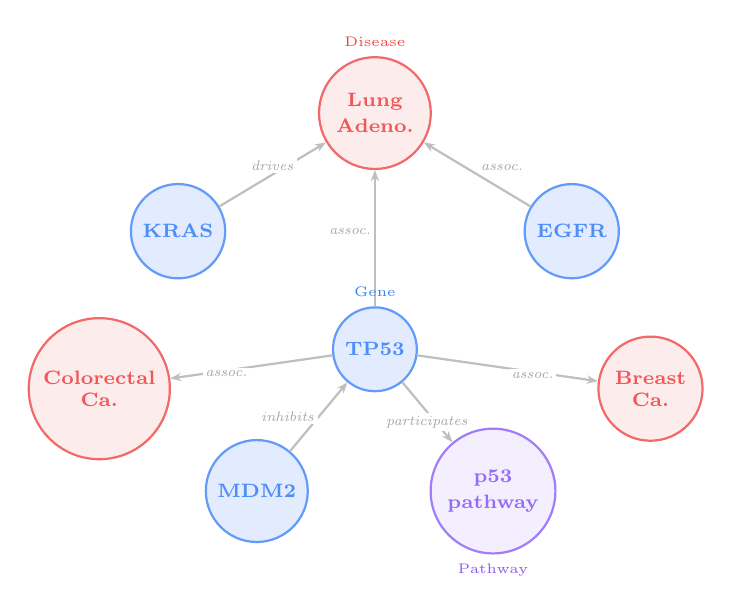
\begin{tikzpicture}[
    gnode/.style={circle, draw=genecol!80, fill=genecol!15, minimum size=0.9cm, font=\scriptsize\bfseries, text=genecol!90, line width=0.8pt},
    dnode/.style={circle, draw=diseasecol!80, fill=diseasecol!10, minimum size=0.9cm, font=\scriptsize\bfseries, text=diseasecol!90, line width=0.8pt},
    pnode/.style={circle, draw=pathwaycol!80, fill=pathwaycol!10, minimum size=0.8cm, font=\scriptsize\bfseries, text=pathwaycol!90, line width=0.8pt},
    edge label/.style={font=\tiny, color=gray!70, midway, fill=white, inner sep=1pt},
    gedge/.style={-{Stealth[length=4pt]}, thick, color=gray!50},
]

% Nodes — gene
\node[gnode] (tp53) at (0,0) {TP53};
\node[gnode] (kras) at (-2.5, 1.5) {KRAS};
\node[gnode] (egfr) at (2.5, 1.5) {EGFR};
\node[gnode] (mdm2) at (-1.5, -1.8) {MDM2};

% Nodes — disease
\node[dnode] (luad) at (0, 3) {\shortstack{Lung\\Adeno.}};
\node[dnode] (brca) at (3.5, -0.5) {\shortstack{Breast\\Ca.}};
\node[dnode] (crc) at (-3.5, -0.5) {\shortstack{Colorectal\\Ca.}};

% Nodes — pathway
\node[pnode] (p53path) at (1.5, -1.8) {\shortstack{p53\\pathway}};

% Edges
\draw[gedge] (tp53) -- node[edge label, above left] {\textit{assoc.}} (luad);
\draw[gedge] (kras) -- node[edge label, above] {\textit{drives}} (luad);
\draw[gedge] (egfr) -- node[edge label, above right] {\textit{assoc.}} (luad);
\draw[gedge] (tp53) -- node[edge label, below right] {\textit{assoc.}} (brca);
\draw[gedge] (tp53) -- node[edge label, below left] {\textit{assoc.}} (crc);
\draw[gedge] (tp53) -- node[edge label, below] {\textit{participates}} (p53path);
\draw[gedge] (mdm2) -- node[edge label, left] {\textit{inhibits}} (tp53);

% Type annotations (direct labels per Saloni)
\node[font=\tiny, color=genecol, anchor=south] at (tp53.north) {Gene};
\node[font=\tiny, color=diseasecol, anchor=south] at (luad.north) {Disease};
\node[font=\tiny, color=pathwaycol, anchor=north] at (p53path.south) {Pathway};

\end{tikzpicture}
\caption{\textbf{Example knowledge graph} for the query ``role of TP53 in cancer.'' Nodes are {\color{genecol}genes} (blue), {\color{diseasecol}diseases} (red), and {\color{pathwaycol}pathways} (purple). Edge labels show extracted relation types. TP53 is the highest-degree hub, connected to three cancer types, a pathway, and a regulatory gene. This graph was enriched by OpenTargets top-10 disease associations for TP53. Node sizes are proportional to $0.4 \times \text{degree} + 0.6 \times \text{confidence}$.}
\label{fig:example_kg}
\end{figure}

\noindent
\textbf{Step~1: Entity extraction.} GLiNER2 identifies \texttt{TP53} (gene, confidence~0.92) and \texttt{cancer} (disease, confidence~0.88) with a \textit{mutated\_in} relation.

\noindent
\textbf{Step~2: KG enrichment.} OpenTargets resolves TP53 to Ensembl ID ENSG00000141510 and returns the top-10 associated diseases including breast carcinoma (score~0.73), colorectal carcinoma (score~0.69), and lung adenocarcinoma (score~0.65). Curated pathway (p53~signaling) and regulatory (MDM2$\rightarrow$TP53) edges are added.

\noindent
\textbf{Step~3: Hypothesis generation.} The system generates two hypotheses: ``TP53 as Driver in Breast Carcinoma'' (confidence~0.82) based on the gene--disease edge weight, and ``p53 Pathway Involvement'' (confidence~0.70) linking TP53 and MDM2 through the shared pathway node.

\noindent
\textbf{Step~4: Parallel retrieval.} Semantic Scholar returns six papers sorted by citation count. CELLxGENE Census provides lung tissue cell metadata (300~cells with cell type and disease annotations).

% ── 6. Limitations ────────────────────────────────────────────────
\section{Limitations}

We believe transparency about limitations is essential for a tool intended for scientific use.

\begin{enumerate}[nosep]
    \item \textbf{No systematic benchmarking.} Hypotheses have not been evaluated against curated ground-truth corpora (e.g., COSMIC, CIViC). We do not report precision, recall, or any quantitative performance metric. The utility of the platform should be evaluated by domain experts on a case-by-case basis.

    \item \textbf{Heuristic hypothesis generation.} Hypotheses are assembled from graph topology (node degree, edge weight) rather than from a trained generative model. Quality varies with query specificity and the coverage of upstream NER and API enrichment.

    \item \textbf{Synthetic atlas data.} UMAP coordinates and expression values in the single-cell atlas view are synthetically generated, not computed from real expression matrices. This module provides metadata browsing, not quantitative analysis.

    \item \textbf{Curated fallback data.} When live APIs (DepMap, GTEx, cBioPortal) are unavailable, the system uses hardcoded reference values for approximately 10~common oncogenes. Users should verify validation results against primary sources.

    \item \textbf{Simplified structural analysis.} Pocket detection uses custom geometry (neighbor density + hierarchical clustering), not established tools such as fpocket or SiteMap. Druggability scoring weights are ad hoc.

    \item \textbf{Simplified gRNA scoring.} Off-target estimation is heuristic (10-mer uniqueness ratio), not based on genome alignment. Researchers should validate guide designs with established tools (e.g., CRISPOR, Benchling).

    \item \textbf{Stateless sessions.} The platform has no user accounts or saved sessions. All queries are independent and cannot be compared or revisited.

    \item \textbf{Oncology-only scope.} Entity schemas, knowledge graph structure, and curated data are tailored to cancer biology. The system does not generalize to other disease areas without modification.
\end{enumerate}

% ── 7. Related Work ───────────────────────────────────────────────
\section{Related Work}

Automated hypothesis generation in biomedicine has been explored through literature-based discovery~\cite{swanson1986fish}, link prediction on biomedical knowledge graphs~\cite{bonner2022review}, and LLM-driven scientific reasoning~\cite{wang2023scientific}.
Onco-TTT differs from these approaches in scope: it is an \emph{integration platform} rather than a novel method, combining zero-shot NER with API-based evidence retrieval into an interactive workflow.

For entity extraction, domain-specific models such as PubMedBERT~\cite{gu2021pubmedbert} and BioBERT~\cite{lee2020biobert} require supervised fine-tuning per entity type. GLiNER2's zero-shot schema composition allows rapid addition of new entity types without retraining.

For hypothesis validation, tools such as Open Targets Genetics, DepMap Portal, and cBioPortal each provide individual evidence dimensions. Onco-TTT's contribution is aggregating these into a single scored dashboard with programmatic access.

% ── 8. Future Work ────────────────────────────────────────────────
\section{Future Work}

Planned improvements include:
\begin{itemize}[nosep]
    \item LLM-powered hypothesis refinement with citation grounding.
    \item Systematic evaluation against CIViC and COSMIC benchmarks.
    \item Real single-cell atlas embeddings via scVI or scArches reference mapping.
    \item Persistent user sessions with hypothesis comparison.
    \item Replacing the graph diffusion heuristic with actual test-time training on the knowledge graph~\cite{sun2024ttt}.
    \item Expansion to additional disease domains.
\end{itemize}

% ── 9. Availability ───────────────────────────────────────────────
\section{Availability}

Onco-TTT is open-source under the MIT license.

\begin{itemize}[nosep]
    \item \textbf{Live demo:} \url{https://onco-hypothesis.up.railway.app}
    \item \textbf{Source code:} \url{https://github.com/inventcures/oncology_hypothesis_generation}
    \item \textbf{Backend API:} \url{https://backend-production-baa6.up.railway.app/docs}
\end{itemize}

% ── Acknowledgments ───────────────────────────────────────────────
\section*{Acknowledgments}

Onco-TTT builds on the work of the GLiNER team (Zaratiana et~al.), the OpenTargets consortium, the Allen Institute for AI (Semantic Scholar), the Chan Zuckerberg Initiative (CELLxGENE Census), the Broad Institute (DepMap), Memorial Sloan Kettering (cBioPortal), the GTEx consortium, and the AlphaFold team at DeepMind.
We gratefully acknowledge these groups for making their tools and data publicly available.

% ── References ────────────────────────────────────────────────────
\begin{thebibliography}{20}

\bibitem{zaratiana2023gliner}
U.~Zaratiana, N.~Golde, and D.~Wangmo.
\newblock GLiNER: Generalist model for named entity recognition using bidirectional transformer.
\newblock \textit{arXiv preprint arXiv:2311.08526}, 2023.

\bibitem{ochoa2023opentargets}
D.~Ochoa, A.~Hercules, B.~M.~Bento, et~al.
\newblock The next-generation Open Targets Platform: reimagined, redesigned, rebuilt.
\newblock \textit{Nucleic Acids Research}, 51(D1):D1353--D1359, 2023.

\bibitem{sun2024ttt}
Y.~Sun, X.~Li, K.~Dalal, et~al.
\newblock Learning to (learn at test time): RNNs with expressive hidden states.
\newblock \textit{arXiv preprint arXiv:2407.04620}, 2024.

\bibitem{kinney2023s2}
R.~Kinney, C.~Anastasiades, R.~Authur, et~al.
\newblock The Semantic Scholar Open Data Platform.
\newblock \textit{arXiv preprint arXiv:2301.10140}, 2023.

\bibitem{czi2023cellxgene}
CZI Single-Cell Biology, et~al.
\newblock CZ CELLxGENE Discover: A single-cell data platform for scalable exploration, analysis and modeling of aggregated data.
\newblock \textit{bioRxiv}, 2023.

\bibitem{jumper2021alphafold}
J.~Jumper, R.~Evans, A.~Pritzel, et~al.
\newblock Highly accurate protein structure prediction with AlphaFold.
\newblock \textit{Nature}, 596:583--589, 2021.

\bibitem{doench2016grna}
J.~G.~Doench, N.~Fusi, M.~Sullender, et~al.
\newblock Optimized sgRNA design to maximize activity and minimize off-target effects of CRISPR-Cas9.
\newblock \textit{Nature Biotechnology}, 34:184--191, 2016.

\bibitem{swanson1986fish}
D.~R.~Swanson.
\newblock Fish oil, Raynaud's syndrome, and undiscovered public knowledge.
\newblock \textit{Perspectives in Biology and Medicine}, 30(1):7--18, 1986.

\bibitem{bonner2022review}
S.~Bonner, I.~P.~Barrett, C.~Ye, et~al.
\newblock A review of biomedical datasets relating to drug discovery: A knowledge graph perspective.
\newblock \textit{Briefings in Bioinformatics}, 23(6):bbac404, 2022.

\bibitem{wang2023scientific}
H.~Wang, J.~P.~Gonzalez-Brenes, et~al.
\newblock Scientific discovery in the age of artificial intelligence.
\newblock \textit{Nature}, 620:47--60, 2023.

\bibitem{gu2021pubmedbert}
Y.~Gu, R.~Tinn, H.~Cheng, et~al.
\newblock Domain-specific language model pretraining for biomedical natural language processing.
\newblock \textit{ACM Transactions on Computing for Healthcare}, 3(1):1--23, 2021.

\bibitem{lee2020biobert}
J.~Lee, W.~Yoon, S.~Kim, et~al.
\newblock BioBERT: a pre-trained biomedical language representation model for biomedical text mining.
\newblock \textit{Bioinformatics}, 36(4):1234--1240, 2020.

\end{thebibliography}

\end{document}
